\chapter{Основные сведения об электромагнитных переходных процессах}
\section{Основные определения}
Из всего многообразия электромагнитных переходных процессов в электрической системе наиболее распространенными являются процессы, вызванные:
\begin{enumerate} 
	\item
	включением и отключением двигателей и других приемников электроэнергии;
	\item
	коротким замыканием в системе, а также повторным включением и отключением (одновременным или 
каскадным) короткозамкнутой цепи;
	\item
	возникновением местной несимметрии в системе (например, отключение одной фазы линии передачи);
	\item
	несинхронным включением синхронных машин. 
\end{enumerate}

\so{Коротким замыканием} называют всякое не предусмотренное нормальными условиями работы замыкание между фазами, а в системах с заземленными нейтралями (или четырехпроводных)~---  также замыкание одной или нескольких фаз на землю (или на нулевой провод).

В системах с незаземленными нейтралями или с нейтралями, заземленными через специальные компенсирующие устройства, замыкание одной из фаз на землю называют \so{простым замыканием}. При этом виде повреждения прохождение тока обусловлено главным образом емкостью фаз относительно земли.

При возникновении короткого замыкания в электрической системе сопротивление цепи уменьшается (степень уменьшения зависит от положения точки короткого замыкания в системе), что приводит к увеличению токов в отдельных ветвях системы по сравнению с токами нормального режима. в свою очередь это вызывает снижение напряжений в системе, которое особенно велико вблизи места короткого замыкания.

Обычно в месте замыкания образуется некоторое переходное сопротивление, состоящее из сопротивления возникшей электрической дуги и сопротивлений прочих элементов пути тока от одной фазы к другой или от фазы на землю. Электрическая дуга возникает или с самого начала происшедшего повреждения как, например, при перекрытии или пробое изоляции, или через некоторое время, когда перегорит элемент, вызвавший замыкание. При замыканиях между фазами переходное сопротивление определяется главным образом сопротивлением электрической дуги.

\begin{wrapfigure}[17]{r}{0.4\linewidth}
	\centering
	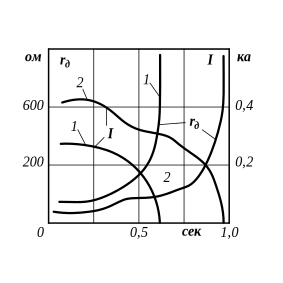
\includegraphics[width=0.95\linewidth]{pic/1-1}
	\caption{Кривые изменения во времени тока и сопротивления самопогасающей открытой дуги на линии 110~\textit{кв} с деревянными опорами. \textit{1, 2} -- номера опытов.}
	\label{fig:r-and-I}
\end{wrapfigure}


Когда токи достаточно велики (сотни ампер и более), сопротивление дуги приблизительно постоянно и по своему характеру почти чисто активное. С уменьшением, тока и увеличением длины дуги, что имеет место в течение переходного процесса, ее сопротивление возрастает. Наглядной иллюстрацией такого изменения могут служить графики (рис.~\ref{fig:r-and-I}), полученные экспериментально при возникновении самопогасающих дуг на линиях 110~\textit{кв} с деревянными опорами.

В ряде случаев переходные сопротивления могут быть столь малы, что практически ими можно пренебречь. Такие замыкания называют \mbox{\so{металлическими}}.

Естественно, при прочих равных условиях ток при металлическом замыкании больше, чем при наличии переходного сопротивления. Поэтому, когда требуется найти возможные наибольшие величины токов, исходят из наиболее тяжелых условий, считая, что в месте замыкания отсутствуют какие-либо переходные сопротивления\footnote{Учет переходных сопротивлений и контактных соединений при выполнении расчетов коротких замыканий для установок напряжением до 1000~\textit{в} имеет особое значение (\colorbox{red}{§ 17-5}).}.

В трехфазных системах с заземленной нейтралью различают следующие основные виды коротких замыканий в одной точке:

\begin{enumerate} 
	\item
	трехфазное;
	\item
	двухфазное;
	\item
	однофазное;
	\item
	двухфазное на землю, т.~е, замыкание между двумя фазами с одновременным замыканием той же точки на землю. 
\end{enumerate}

Трехфазное короткое замыкание является симметричным, так как при нем все фазы остаются в одинаковых условиях\footnote{При наличии переходных сопротивлений симметрия сохраняется лишь при равенстве этих сопротивлений.} Напротив, все остальные виды коротких замыканий являются несимметричными, поскольку при каждом из них фазы находятся уже в неодинаковых условиях; поэтому системы токов и напряжений при этих видах короткого замыкания в той или иной мере искажены.
	
Многолетняя аварийная статистика по союзным и зарубежным системам показывает, что при глухозаземленной нейтрали относительная вероятность различных основных видов короткого замыкания характеризуется примерными данными табл. \colorbox{red}{1-1} В той же таблице показаны рекомендуемые сокращенные обозначения каждого вида короткого замыкания.

Как видно из этой таблицы, подавляющее число коротких замыканий связано с замыканием на землю, в то время как трехфазное короткое замыкание является очень редким. Однако отсюда было бы неправильным делать вывод, что трехфазное короткое замыкание можно вообще оставить без внимания. Поскольку оно все же возможно, с ним следует считаться, тем более что оно иногда может быть решающим для окончательного суждения относительно возможности работы в условиях короткого замыкания. Само изучение процесса трехфазного короткого замыкания особенно важно в связи с тем, что применение метода симметричных составляющих позволяет величины токов и напряжений прямой последовательности любого несимметричного замыкания определять как соответственные величины при некоторых условных трехфазных замыканиях.

\begin{table}[h]
	\centering
	\begin{tabular}{|>{\centering\arraybackslash}m{0.2\linewidth}|>{\centering\arraybackslash}m{0.32\linewidth}|>{\centering\arraybackslash}m{0.19\linewidth}|>{\centering\arraybackslash}m{0.19\linewidth}|}
		\hline
		Виды короткого замыкания & Принципиальная схема & Буквенное обозначение на схемах места и вида короткого замыкания & Относительная вероятность короткого замыкания, \% \\
		\hline
		Трехфазное & 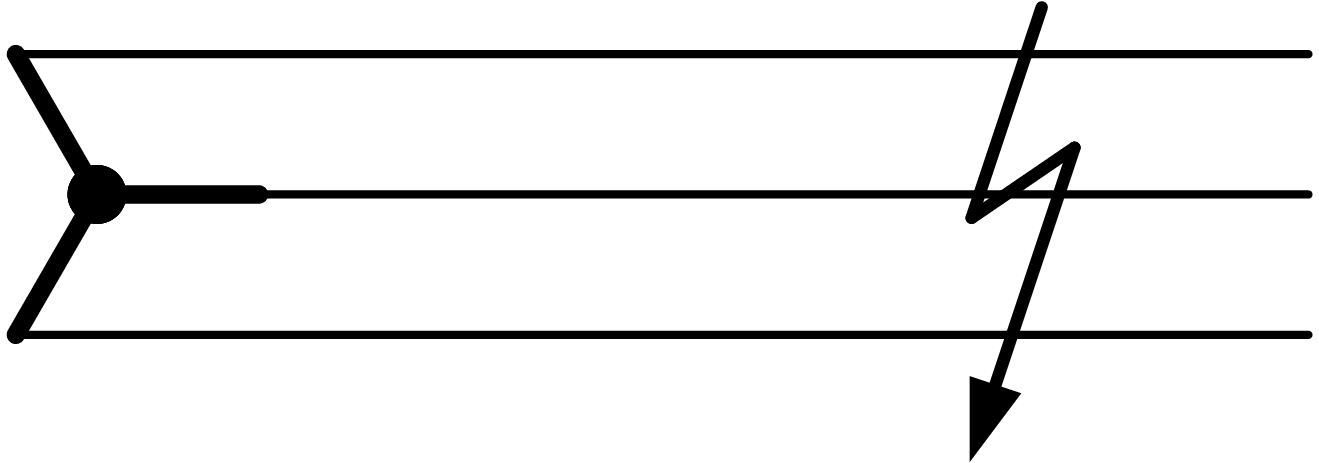
\includegraphics[width=0.7\linewidth]{pic/1-2-1} & $ K^{(3)} $ & 5 \\
		Двухфазное & 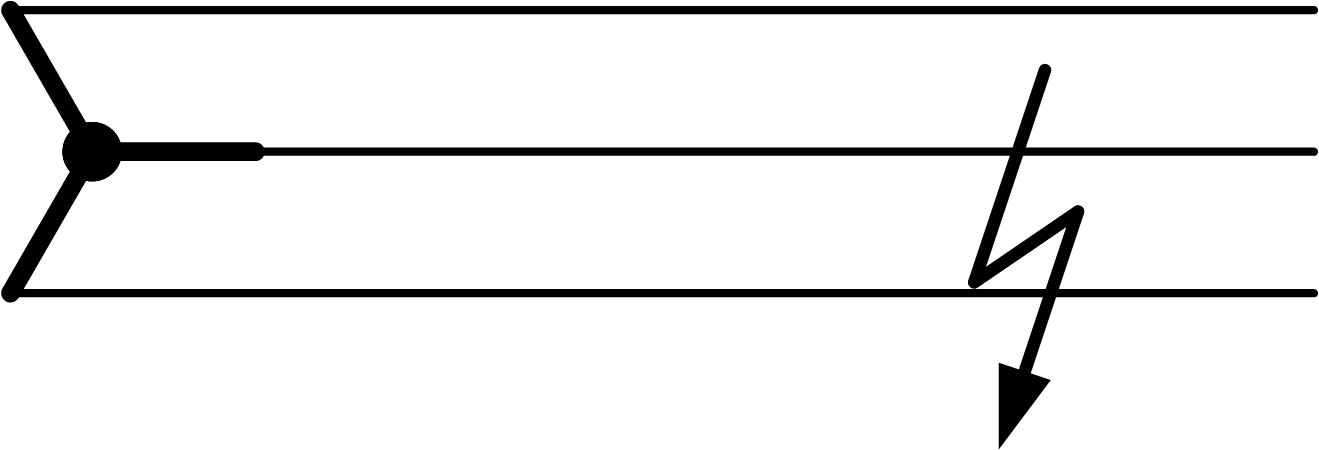
\includegraphics[width=0.7\linewidth]{pic/1-2-2} & $ K^{(2)} $ & 10 \\
		Однофазное & 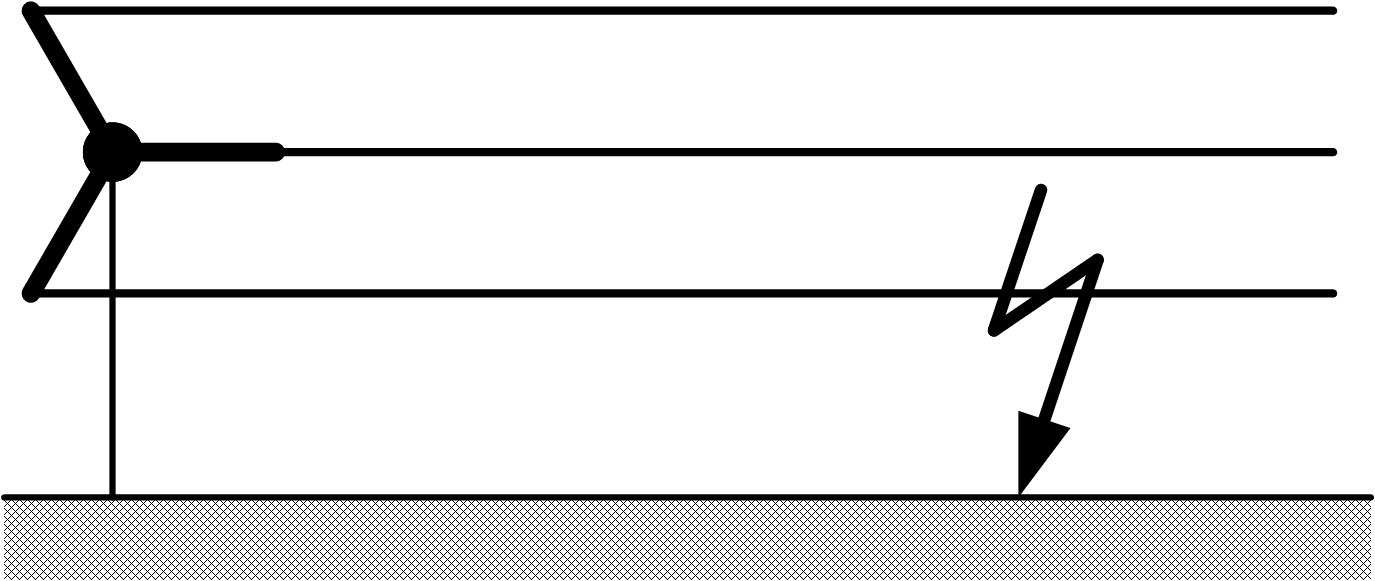
\includegraphics[width=0.7\linewidth]{pic/1-2-3} & $ K^{(1)} $ & 65 \\
		Двухфазное на землю & 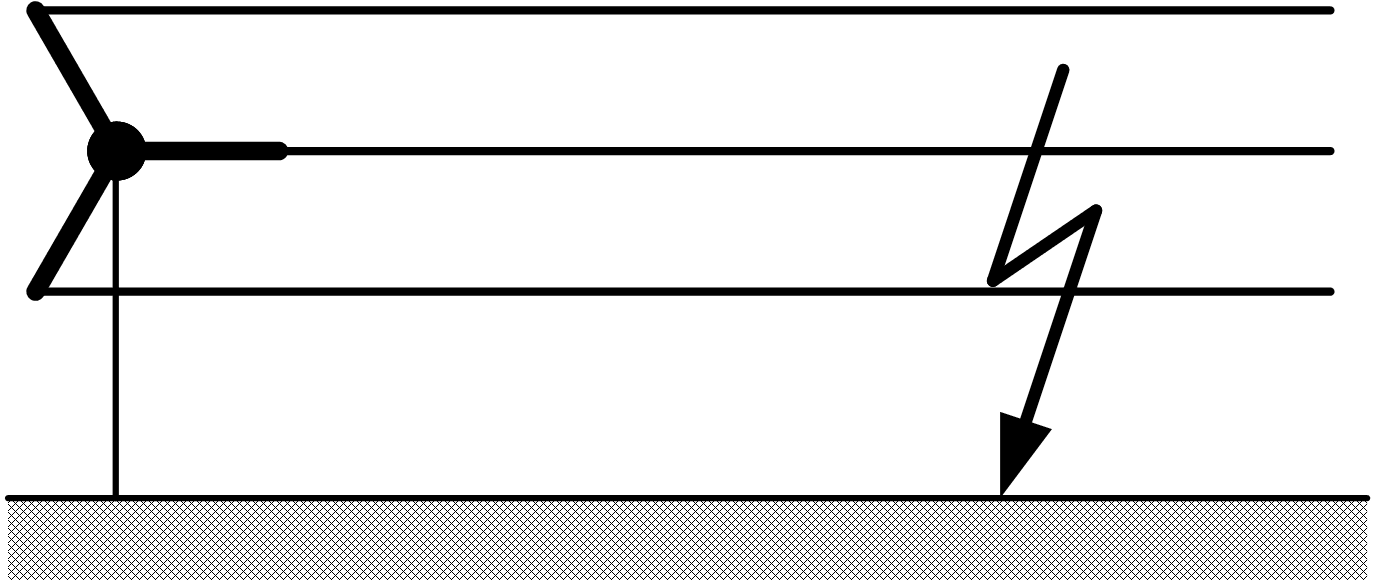
\includegraphics[width=0.7\linewidth]{pic/1-2-4} & $ K^{(1,1)} $ & 20 \\
		\hline
	\end{tabular}
	\caption{Относительная вероятность и сокращенные обозначения основных видов короткого замыкания}
	\label{tabl:veroiatnost-kz}
\end{table}

Здесь нелишне также отметить, что процесс включения любого трехфазного приемника или невозбужденного синхронного генератора или двигателя можно рассматривать как трехфазное короткое замыкание за некоторым сопротивлением.

Иногда в процессе развития аварии первоначальный вид короткого замыкания переходит в другой вид короткого замыкания. Так, например, в кабельных сетях (с трехжильными кабелями) несимметричные короткие замыкания часто переходят в трехфазные короткие замыкания, так как образовавшаяся при повреждении в кабеле электрическая дуга быстро разрушает изоляцию между его жилами.

Несимметричные короткие замыкания, а также несимметричные нагрузки по существу представляют различные виды \so{поперечной несимметрии}.

Нарушение симметрии какого-либо промежуточного элемента трехфазной цепи (например, отключение одной фазы линии передачи и т.~п.) называют \so{продольной несимметрией}.

Возможны случаи, когда одновременно возникает несколько несимметрий одинакового или различного вида. Так, например, при обрыве провода воздушной линии один его конец, расположенный близко к точке подвеса, остается изолированным, а другой, упав на землю, образует однофазное короткое замыкание. Здесь одновременно возникают продольная и поперечная несимметрии. В качестве другого примера, когда возникают несимметрии одного вида, может служить так называемое \so{двойное замыкание на землю}, т.~е. одновременное замыкание на землю разных фаз в различных точках сети, работающей с изолированной нейтралью.

Все виды повреждений, сопровождающихся мног кратной несимметрией, называют \so{сложными}. К ним, очевидно, относится также любое несимметричное короткое замыкание в сети, работающей в неполнофазном режиме.

Практикой \colorbox{red}{эксплуатации} электрических систем установлено, что большая часть возникающих повреждений, особенно на воздушных линиях, имеет проходящий характер, т.~е. повреждения самоустраняются после отключения поврежденного участка и не возникают вновь при обратном включении его. Примером такого самоустраняющегося повреждения может служить обычное перекрытие по поверхности гирлянды изоляторов линии, вызванное грозовым разрядом. После отключения линии электрическая прочность воздушного промежутка восстанавливается в течение небольшого отрезка времени, необходимого для деионизации воздуха в месте перекрытия.

В соответствии с этим широкое применение нашло автоматическое повторное включение (АПВ) цепей и особенно воздушных линий. Поскольку на последних преобладают замыкания одной фазы, у них производят иногда отключение только поврежденной фазы с после дующим однофазным автоматическим повторным включением (ОАПВ). Наконец, помимо однократного выполняют также многократное автоматическое повторное включение с соответствующими интервалами времени его действия.

Наглядной иллюстрацией эффективности автоматического повторного включения служат данные табл.~\colorbox{red}{1-2}, представляющие показатели работы устройств автоматического повторного включения по всем союзным энергосистемам за пятилетие 1962—1966~гг. \colorbox{red}{[Л. 14]}.

Как видно, на воздушных линиях относительное число самоустраняющихся повреждений, которому соответствует успешная работа автоматического повторного включения, составляет значительное большинство (преимущественно у линий 20—330~\textit{кв}) всех повреждений на них, причем успешная работа АПВ многократного действия несколько выше, чем однократного действия. Последнее указывает на то, что для самоустранения повреждения иногда требуется больше времени, чем интервал до первого повторного включения.

В кабельных линиях, как и следовало ожидать, число самоустраняющихся повреждений заметно меньше, чем в воздушных. Оно составляет примерно половину общего числа повреждений в кабелях.

Интересно отметить, что даже у трансформаторов больше половины всех повреждений являются самоустраняющимися.

При неуспешном автоматическом повторном включении, т.~е. когда возникшее повреждение в цепи сохранилось, переходный процесс состоит из нескольких этапов. Первый из них наступает в момент возникновения короткого замыкания и продолжается до отключения поврежденного участка. Вторым этапом является пауза (порядка 0,5~\textit{сек} и более) до момента повторного включения, с которого наступает третий этап, продолжающийся до нового отключения того же участка. При многократном автоматическом повторном включении число этапов соответственно возрастает\footnote{Пауза перед вторым повторным включением значительно больше, чем перед первым таким включением. Она определяется характеристиками самого выключателя.}. При применении однофазного автоматического повторного включения в течение паузы перед повторным включением в системе сохраняется местная продольная несимметрия (отключена одна фаза).


